\chapter{Korrelierte Messgrössen}
\label{chap:korrelation}

\begin{center}
\begin{tcolorbox}[enhanced,width=6in,center upper,
    fontupper=\large,drop fuzzy shadow southwest,
    colframe=blue!50!black,colback=blue!10]
Für dieses Kapitel ist ein Jupyter-Notebook verfügbar. Siehe \gitresource{Kovarianz.ipynb} 
\end{tcolorbox}
\end{center}

Bislang haben wir in unseren Beispielen immer nur eine einzige Zufallsvariable gemessen oder Fälle betrachtet, in denen alle Zufallsvariablen voneinander unabhängig waren. In realen Experimenten treten allerdings häufig Korrelationen der Messgrössen auf. In diesem Fall geht eine Änderung in einer Variable mit einer Änderung der anderen Variable einher. Zum Beispiel könnte die Frequenz eines Resonators mit der Raumtemperatur korreliert sein. Eine derartige Korrelation muss in die Fehleranalyse einbezogen werden, wie wir in Gleichung \ref{eq:Gauss2D} sehen. \\

Bei der Analyse und Interpretation der Korrelation ist allerdings Vorsicht geboten: Korrelation wird häufig verwendet, um einen kausalen Zusammenhang aufzuzeigen. Allerdings bedeutet das Vorliegen einer Korrelation zweier Variablen $x$ und $y$ nicht automatisch, dass ein kausaler Zusammenhang zwischen ihnen besteht. Zwei Variablen $x$ und $y$ können etwa indirekt durch eine dritte Variable $z$ verbunden sein. Wenn $z$ sowohl $x$ als auch $y$ beeinflusst, können letztere eine Korrelation aufweisen, ohne dass sie direkt kausal verbunden sind. In unserem Beispiel des Resonators könnte zum Beispiel die Luftfeuchtigkeit im Raum der Grund dafür sein, dass sowohl die Temperatur als auch die Frequenz ansteigen oder abfallen.

\section{Kovarianz}
\label{chap:korrelation:sec:kovarianz}

Um einen linearen Zusammenhang zwischen zwei Variablen aufzuzeigen, verwenden wir die geschätzte Kovarianz
\begin{align}
\gls{gl:cov}(x,y) = \frac{1}{N - 1} \sum_{n = 1}^N (x_n - \overline{x})(y_n - \overline{y})\,.
\label{eq:Kovarianz}
\end{align}
In Messungen mit vielen Datenpunkten (mit $\frac{1}{N-1}\rightarrow \frac{1}{N}$) wird diese Formel häufig vereinfacht zu:
\begin{align}
\sigma_{xy}^2 = \text{cov}(x,y) = \frac{1}{N} \sum_{n = 1}^N (x_n - \overline{x})(y_n - \overline{y}).
\label{eq:Kovarianzsimple}
\end{align}
Die Kovarianz hat die Einheit $[\sigma_{xy}^2]=[x]\times[y]$. Damit hängt der Wert der Kovarianz von den gewählten Einheiten ab und hat keine universelle Bedeutung. Beispielsweise ändert sich der Zahlenwert einer Kovarianz, wenn wir Nanometer statt Meter als Längeneinheit festlegen. Um eine einheitenlose Zahl mit einer universellen Bedeutung zu erhalten, definieren wir den normalisierten Korrelationskoeffizienten:
\begin{align}
\gls{gl:rhoxy} = \frac{ \text{cov} (x,y) }{ \sigma_x \sigma_y } \quad \in [-1,1]\,.
\label{eq:Korrelationskoeffizient}
\end{align}

Hierbei bedeutet:
\begin{align}
\rho_{xy} = 
    \begin{cases}
        0,& \text{unkorrelierte Variablen}\\
        \pm 1,& \text{maximal (anti-)korrelierte Variablen für $y =  ax$.}
    \end{cases}       
\end{align}

Die Varianzen und Kovarianzen können kompakt in der sogenannten Kovarianz-Matrix zusammengefasst werden, die Sie bereits in Anschnitt \ref{chap:fehler:sec:fehlerfortpflanzung} kennengelernt haben:
\begin{align}
\begin{pmatrix}
\sigma_x^2    & \sigma_{xy}^2 & \cdots \\
\sigma_{yx}^2 & \sigma_y^2    & \cdots \\
\vdots        & \vdots        & \ddots \\
\end{pmatrix}\,.
\end{align}

Wie oben bereits erwähnt, misst die Kovarianz allerdings nur lineare Korrelationen, nichtlineare Fälle müssen anders behandelt werden. Um das zu verdeutlichen, berechnen wir die Kovarianz für die nichtlineare Funktion $y = x^2$. Hier sei $x$ eine Zufallsvariable mit einer symmetrischen Verteilungsfunktion, das heisst $-x$ ist gleich wahrscheinlich wie $x$. Für die Kovarianz erhalten wir 
\begin{align}
    \begin{split}
        \text{cov}(x,y) &= \frac{1}{N} \sum_{n = 1}^N ( x_n - \overline{x} )( y_n - \overline{y} )\\
        &= \frac{1}{N} \sum_{n = 1}^N x_n ( x_n^2 - \overline{y} )\\
        &= \frac{1}{N} \sum_{n = 1}^N x_n^3  - \frac{1}{N} \sum_{n = 1}^N x_n \overline{y} = 0 \quad \text{f\"ur } N \rightarrow{ \infty} \, ,
    \end{split}
\end{align}
was verdeutlicht, dass nichtlineare Korrelationen mit erweiterten Methoden untersucht werden müssen. \\

Wir wollen lineare Korrelationen nun am Beispiel von einfachen trigonometrischen Funktionen veranschaulichen. Hierzu generieren wir zunächst drei künstliche, quasi analoge Signale $U_1$, $U_2$ und $U_3$. Die Signale $U_1$ und $U_3$ sind Sinusfunktionen verschiedener Amplituden, aber gleicher Frequenzen. Signal $U_2$ ist eine Kosinusfunktion mit gleicher Amplitude und Frequenz wie $U_1$. Alle Signale werden mit identischem Rauschen überlagert. 


\begin{lstlisting}[language = Python]

N = 1001 # Laenge des Datenvektors
t = np.linspace(0, N-1, N) # Zeitvektor von Punkten mit Abstand 1 in Einheit von Nanosekunden (als konkretes Beispiel)

f_sig = 0.01 # Frequenz 
Amp1 = 1.2 # Amplitude 1
Amp3 = 5.2 # Amplitude 2 
sig1 = Amp1*np.sin(2*np.pi*f_sig*t) # Signal  1  
sig2 = Amp1*np.cos(2*np.pi*f_sig*t) # Signal 2
sig3 = Amp3*np.sin(2*np.pi*f_sig*t)  # Signal 3  
noise_amp = 0.2 # Amplitude des Rauschens
noise1 = np.random.normal(0,noise_amp,N) # normalverteiltes Rauschen mit Standardabweichung noise_amp
noise2 = np.random.normal(0,noise_amp,N) # normalverteiltes Rauschen mit Standardabweichung noise_amp
noise3 = np.random.normal(0,noise_amp,N) # normalverteiltes Rauschen mit Standardabweichung noise_amp
U1 = sig1 + noise1 # addiere Rauschen zu Signal 1
U2 = sig2 + noise1 # addiere Rauschen zu Signal 2
U3 = sig3 + noise1 # addiere Rauschen zu Signal 3
\end{lstlisting}

In einem ersten Schritt können wir diese Daten nun einfach visualisieren (siehe Figur \ref{fig:Us}). Diese Darstellung lässt bereits erahnen, dass $U_1$ und $U_3$ korreliert sind, doch vor allem für  $U_1$ und $U_2$ ist aus dieser Darstellung nur schwer ersichtlich, ob tatsächlich eine Korrelation vorliegt. 

\begin{figure}[H]
\centering
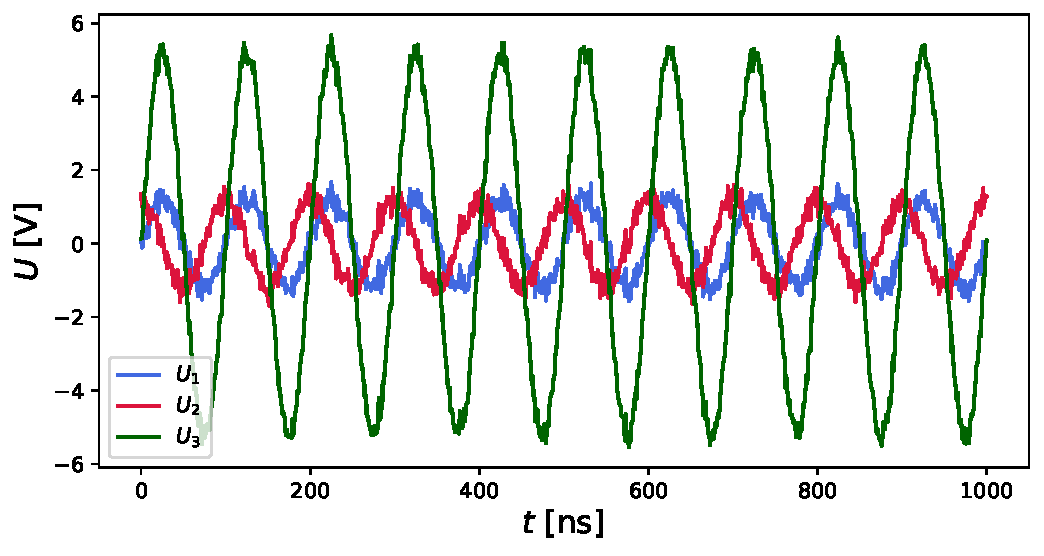
\includegraphics[width=0.75\textwidth]{Figures/Usplot.pdf}
\caption{Visualisierung der künstlich generierten, quasi-analogen und rauschbehafteten Signale $U_1$. $U_2$ und $U_3$ als Funktion der Zeit $t$.}
\label{fig:Us}
\end{figure}

Zur graphischen Überprüfung linearer Korrelation stellen wir nun $U_2$ und $U_3$ als Funktion von $U_1$ dar (siehe Figur \ref{fig:korrUs}). Aus dieser Darstellung ist direkt ersichtlich, dass $U_1$ und $U_3$ stark korreliert sind, $U_1$ und $U_2$ hingegen nur sehr schwach. Diese schwache Korrelation von $U_1$ und $U_2$ kommt dadurch zustande, dass beiden Signalen identisches Rauschen anhaftet. 

\begin{figure}[H]
\centering
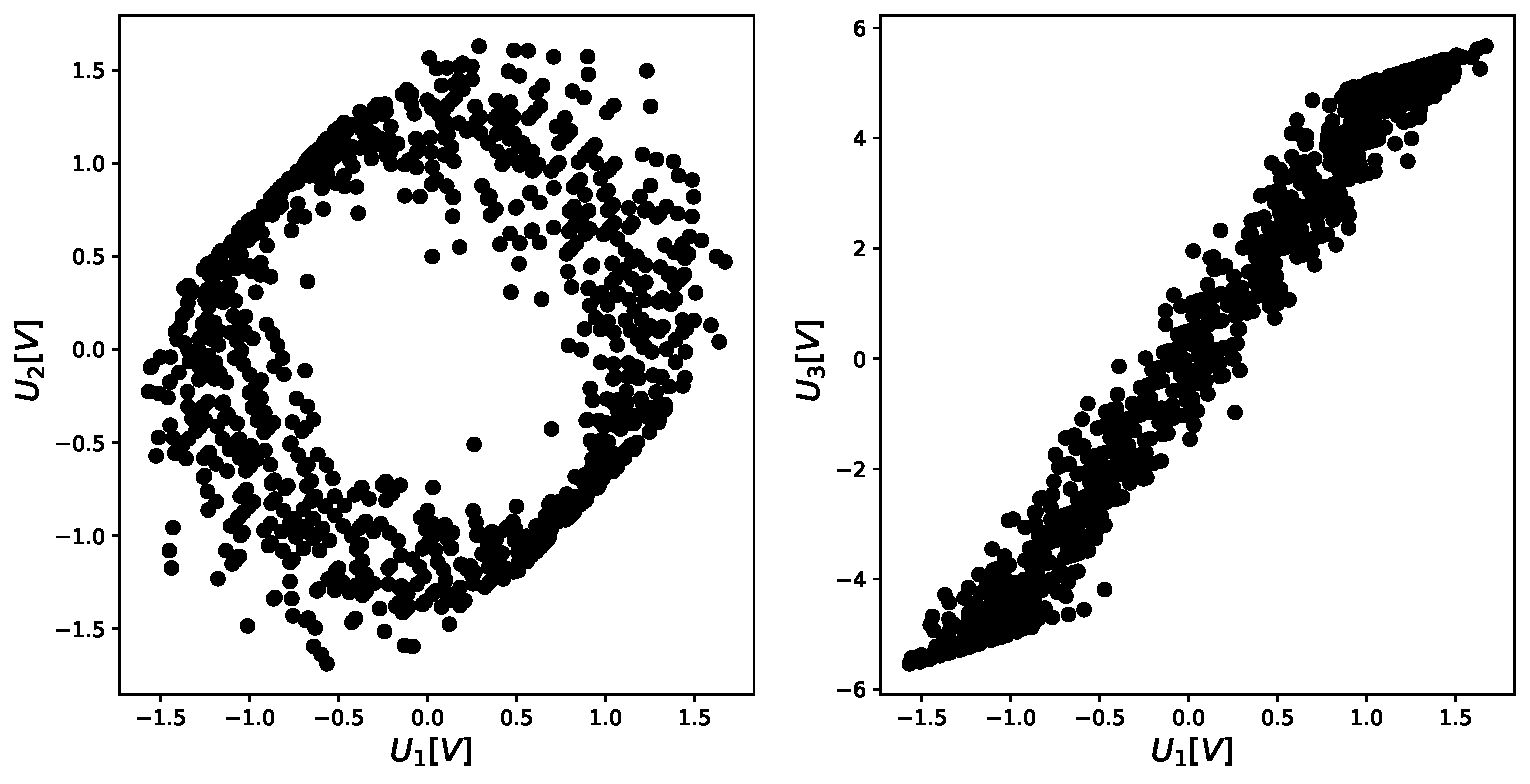
\includegraphics[width=0.75\textwidth]{Figures/Uskorrplot.pdf}
\caption{Um eine möglich Korrelation zwischen zwei Variablen graphisch zu überprüfen, stellt man die eine Variable als Funktion der anderen dar. \textbf{Links:} $U_2$ als Funktion von $U_1$. Die Punkte liegen nicht auf einer Geraden, es liegt also keine starke lineare Korrelation vor. \textbf{Rechts:} $U_3$ als Funktion von $U_1$. Wir sehen eine starke, lineare Korrelation der beiden Variablen.}
\label{fig:korrUs}
\end{figure}
Wir berechnen nun die oben eingeführte Kovarianz sowie die normalisierten Korrelationskoeffizienten.

\begin{lstlisting}[language = Python]
# U1 U3 
C = np.stack((U1,U3), axis=0)
cov13 = np.cov(C)
corcov13 = np.corrcoef(C)

# U1 U2
D = np.stack((U1, U2), axis = 0)
cov12 = np.cov(D)
corcov12 = np.corrcoef(D)
\end{lstlisting}

Die so erhaltenen Korrelationskoeffizienten $\rho_{U_1, U_2}=0.06$ und $\rho_{U_1, U_3}=0.98$ stützen unsere anfängliche, qualitative Analyse. \\

Als nächstes simulieren wir die Messung unserer quasi-analogen Signale mit einem rauschbehafteten Analog-Digital-Konvertierer (engl: Analog-Digital-Converter ADC). Das so hinzugefügte Rauschen ist nun für jedes Signal unterschiedlich. 
\begin{lstlisting}[language = Python]
Delta_t = 1 # zeitl. Abstand der Messpunkte in den gewaehlten Einheiten: fuer einen Zeitvektor t mit Abstaenden von je 1 Nanosekunde misst unser ADC einen Datenpunkt alle Delta_t Nanosekunden
U_max = 10 # maximal messbarer Wert: alle groesseren Werte werden als U_max angezeigt (clipping)
U_min = 0.01 # minimaler messbarer Spannungsunterschied der Signalwerte: Spannungsaufloesung des ADC
U_noise = 1 # Standardabweichung des Spannungsrauschens, das dem Signal durch den Messprozess hinzugefuegt wird

# Initialisierung der Messvektoren
n_mess = math.floor(N/Delta_t)-1 # Anzahl gemessener Punkte. floor rundet ab
n = range(n_mess) # wird fuer for loop benoetigt, enthaelt 0 und n_mess als untere und obere Grenze von n
t_mess = np.zeros(n_mess) # leerer Vektor, um die Zeitwerte zu erfassen
U1_mess = np.zeros(n_mess) # leerer Vektor, um die Spannungswerte zu erfassen
U2_mess = np.zeros(n_mess) # leerer Vektor, um die Spannungswerte zu erfassen
U3_mess = np.zeros(n_mess) # leerer Vektor, um die Spannungswerte zu erfassen

for i in n:
    t_mess[i] = t[(i+1)*Delta_t] # jeder (i+1)*Delta_t-te Punkt wird gemessen
    U1_mess[i] = np.clip(U_min*round((U1[(i+1)*Delta_t]+np.random.normal(0,U_noise))/U_min,0),-U_max,U_max) # numpy.clip limitiert die maximalen Werte auf [-U_max,U_max]
    U2_mess[i] = np.clip(U_min*round((U2[(i+1)*Delta_t]+np.random.normal(0,U_noise))/U_min,0),-U_max,U_max) # numpy.clip limitiert die maximalen Werte auf [-U_max,U_max]
    U3_mess[i] = np.clip(U_min*round((U3[(i+1)*Delta_t]+np.random.normal(0,U_noise))/U_min,0),-U_max,U_max) # numpy.clip limitiert die maximalen Werte auf [-U_max,U_max]
\end{lstlisting}
Wir können die so erhaltenen, ``gemessenen'' Signale $U_1^{\mathrm{mess}}$, $U_2^{\mathrm{mess}}$ und $U_3^{\mathrm{mess}}$ nun erneut als Funktionen der Zeit $t$ als auch als Funktionen von $U_1^{\mathrm{mess}}$ darstellen. 

\begin{figure}[H]
\centering
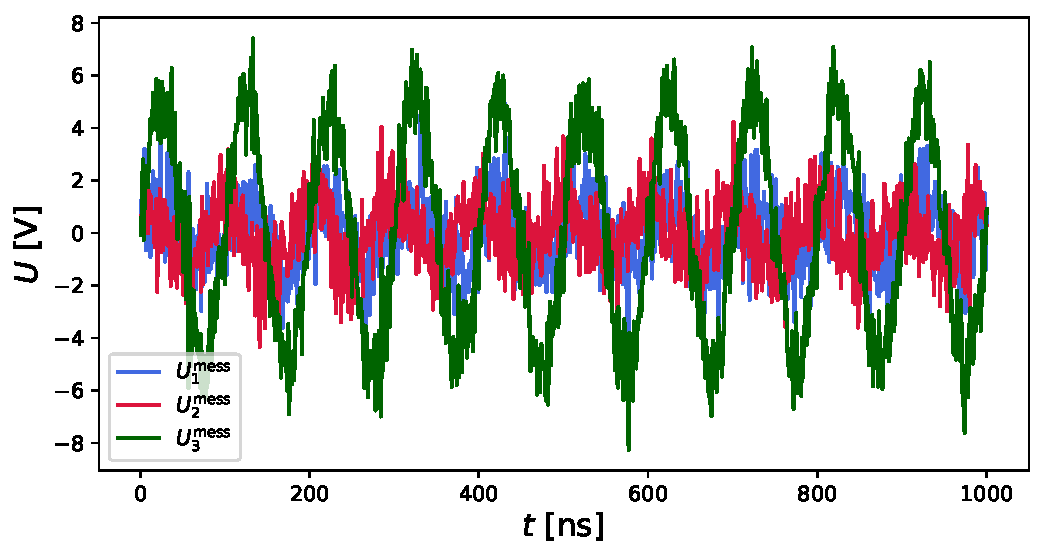
\includegraphics[width=0.75\textwidth]{Figures/Umess.pdf}
\caption{Visualisierung der künstlich generierten Signale $U_1^{\mathrm{mess}}$, $U_2^{\mathrm{mess}}$ und $U_3^{\mathrm{mess}}$ nach der Messung mit einem rauschbehafteten ADC  als Funktion der Zeit $t$.}
\label{fig:Umess}
\end{figure}

Sowohl die Darstellung in Abbildung~\ref{fig:Umesskorr} als auch die erneute Berechnung der Korrelationskoeffizienten zu $\rho_{U_1^{\mathrm{mess}}, U_2^{\mathrm{mess}}}=0.05$ und $\rho_{U_1^{\mathrm{mess}}, U_3^{\mathrm{mess}}}=0.63$ ergeben, dass das Hinzufügen dieses unkorrelierten Rauschens die Korrelation der Signale reduziert hat. Dieses einfache Beispiel verdeutlicht, dass in einem realen Messvorgang Korrelationen einzelner Variablen durch zu starkes Rauschen reduziert, bzw. vollkommen maskiert werden können.


\begin{figure}[H]
\centering
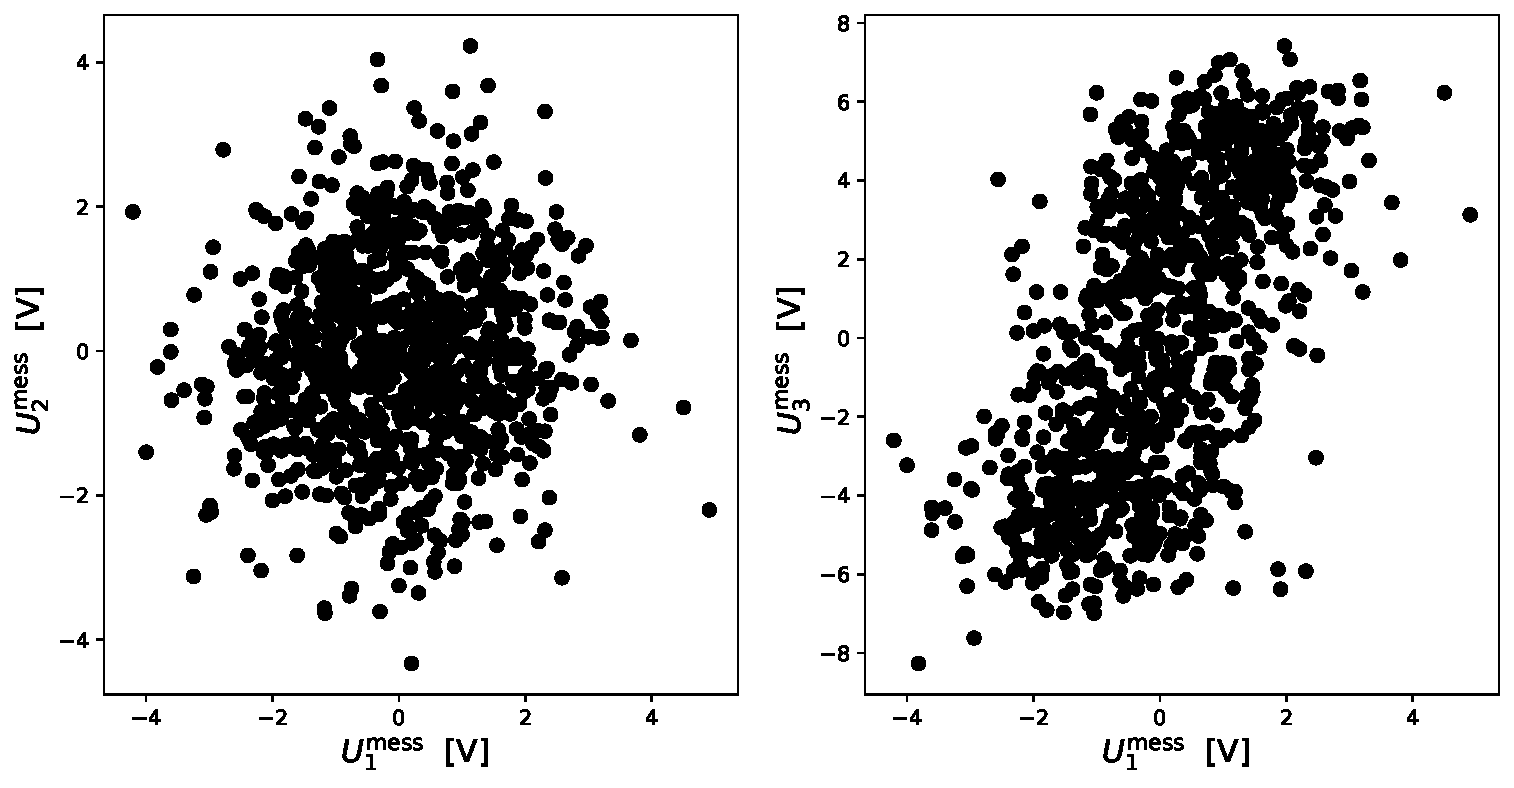
\includegraphics[width=0.75\textwidth]{Figures/Umesskorrplot.pdf}
\caption{Korrelationen zwischen den Signalen, nachdem sie von einem simulierten ADC (mit Rauschen) gemessen wurden.\textbf{Links:} $U_2^{\mathrm{mess}}$ als Funktion von $U_1^{\mathrm{mess}}$. \textbf{Rechts:} $U_3^{\mathrm{mess}}$ als Funktion von $U_1^{\mathrm{mess}}$.}
\label{fig:Umesskorr}
\end{figure}

Wir fassen zusammen: Ob zwei Signale korreliert sind oder nicht, ist nicht davon abhängig, ob sie Rauschen enthalten. Korrelation (selbst starke) kann beispielsweise durch korreliertes Rauschen entstehen. Gleichzeitig müssen rauschfreie Signale nicht korreliert sein, selbst wenn sie, wie in Abbildung~\ref{fig:Us}, dieselbe Frequenz haben.


\section{Auto-Kovarianz}
\label{chap:korrelation:sec:autokovarianz}


%Setzt man in \cref{eq:covariancesimplified} $y = x$ ein, erhält man die Varianz:
%\begin{align}
%\text{cov}(x,x) = \frac{1}{N} \sum_{n = 1}^N (x_n - \overline{x})^2 = \text{var} (x) = \sigma_x^2.
%\end{align}
Häufig sollen nicht zwei verschiedene Messgrössen miteinander korreliert werden, sondern eine Messgrösse mit sich selbst in Abhängigkeit einer Zeitverschiebung. Durch Einsetzen von $y = x_{i+\Delta}$ in Gleichung \ref{eq:Kovarianz}  erhält man die diskrete Auto-Kovarianz, also die Korrelation der Funktion $x$ mit sich selber in Abhängigkeit einer Indexverschiebung $\Delta$
\begin{align}
\gls{gl:RxxDelta} = \frac{1}{N} \sum_{n = 1}^N (x_n - \overline{x})(x_{n+\Delta} - \overline{x}). \label{eq:AutokovarianzDeskret}
\end{align}

Analog zum Korrelationskoeffizienten definieren wir den Autokorrelationskoeffizienten
\begin{align}
\gls{gl:rhoxx} = \frac{ R_{xx} (\Delta) }{ \sigma_x^2 } \quad \in [-1,1]\,.
\end{align}
In vielen Anwendungen sind wir an der diskreten Autokovarianz als Funktion der Zeitverschiebung $\tau = \Delta \times \delta t$ interessiert und verwenden diese Zeitverschiebung anstelle der Indexverschiebung als Variable, sodass wir 
\begin{align}
R_{xx} (\tau) = \frac{1}{N} \sum_{t = t_1}^{t_N} (x(t) - \overline{x})(x(t + \tau) - \overline{x})
\end{align}
mit dem entsprechenden Autokorrelationskoeffizienten:
\begin{align}
\rho_{xx} = \frac{ R_{xx} (\tau) }{ \sigma_x^2 } \quad \in [-1,1]\,.
\end{align}
erhalten. \\

Theoretisch existiert für kontinuierliche Funktionen auch die kontinuierliche Auto-Kovarianz
\begin{align}
\gls{gl:Rxxtau} = \lim_{T \rightarrow \infty} \frac{1}{T} \int_0^T x(t) x(t + \tau) dt = \langle x(t) x(t + \tau) \rangle \,.
\end{align}
Diese kann allerdings nicht für diskrete Signale verwendet werden und ist daher in realen Anwendungen nicht von Relevanz. Wichtige Eigenschaften der Auto-Kovarianz sind wie folgt:
\begin{itemize}
    \setlength\itemsep{0em}
        \item Die Auto-Kovarianz ist symmetrisch um $\Delta = 0$ (bzw. $\tau = 0$).
        \item Die Samplingzeit \gls{gl:deltat} (zeitlicher Abstand zwischen aufeinanderfolgenden Messpunkten) setzt ein unteres Limit für die zeitliche Auflösung der Messung, und damit für die `periodische Zeit' $\tau$.
        \item Die Auto-Kovarianz bei $\Delta = 0$ ($\tau = 0$) entspricht der Varianz und ist das Maximum der Funktion.
        \item Die Auto-Kovarianz von Gauss-verteiltem weissen Rauschen ist Null f\"ur alle $\tau \neq 0$, da weisses Rauschen per Definition von Punkt zu Punkt vollkommen unkorreliert ist.
        \item Die Auto-Kovarianz einer perfekten Sinuswelle ist als Funktion von $\tau$ perfekt periodisch, da Punkte über jede Periode (und damit über jedes ganzzahlige Mehrfache der Periode) perfekt korreliert sind.
\end{itemize}

Die Auto-Kovarianz ist geeignet, um periodische zeitliche Zusammenhänge zu sehen. Ein typisches Beispiel ist die Bestimmung der Korrelationszeit (``Kohärenzzeit'') aus der Breite des Maximums um $\tau = 0$. Aperiodische zeitliche Information (wie z.B. ein kurzer Signalpuls) ist darin aber nicht mehr sichtbar.

Wir wollen nun für unser im Kovarianz-Kapitel eingeführtes Test-Signal $U_1$ die Auto-Kovarianz berechnen. Hierfür definieren wir zunächst die entsprechende Auto-Kovarianzfunktion und wenden diese auf $U_1$ an.
\begin{lstlisting}[language = Python]
# definiere Auto-Kovarianzfunktion
def Rxx(x, delta):
    xm = np.mean(x)
    dev_sum = 0
    for i in range(len(x) - delta):
        dev_sum += (x[i] - xm) * (x[i + delta] - xm)
    return dev_sum / (len(x) - delta)

# wende Funktion auf Beispiele an 
delta_max = len(U1)
Rxx_vs_delta = [Rxx(U1, i) for i in range(delta_max)]
lags = np.linspace(0, delta_max, num=delta_max)
\end{lstlisting}
Da $U_1$ eine Sinusfunktion ist,  erreicht die Auto-Kovarianzfunktion in periodischen Abständen Maxima und Minima (siehe   \ref{fig:AutokorrelationU1}). Wenn $\Delta$ dem Vielfachen einer Periode von $U_1$ entspricht, liegt eine hohe Korrelation vor, nach ungeraden Vielfachen einer halben Periode von $U_1$ eine hohe Anti-Korrelation.   
\begin{figure}[H]
\centering
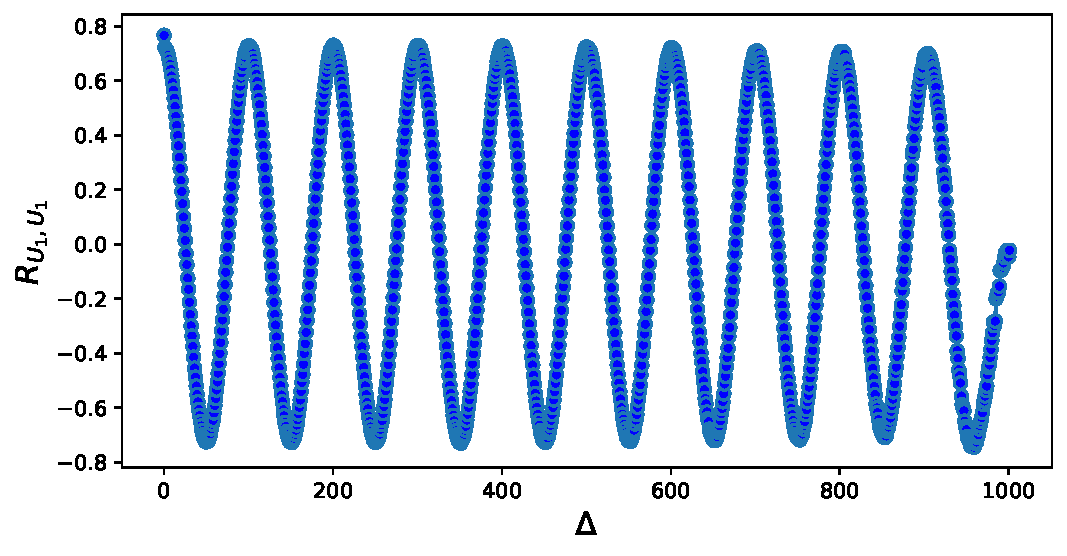
\includegraphics[width=0.75\textwidth]{Figures/U1Auto.pdf}
\caption{Autokorrelationsfunktion $R_{U_1U_1}(\Delta)$ von $U_1$ als Funktion der Indexverschiebung $\Delta$.}
\label{fig:AutokorrelationU1}
\end{figure}




\begin{center}
\begin{tcolorbox}[enhanced,width=6in,drop fuzzy shadow southwest,
colframe=blue!50!black,colback=blue!01]
\textbf{Anwendungsbeispiel}: Ultraschnelle Laserphysik \\
Ein reales Anwendungsgebiet der  Autokorrelation ist die  ultraschnelle Laserphysik (Engl: Ultrafast Laser Physics). Die Charakterisierung von ultraschnellen optischen Pulsen gestaltet sich häufig  schwierig, weil die verfügbaren elektrischen Techniken nur über eine limitierte Zeitauflösung (1-10 Picosekunden) verfügen, die Dauer der Pulse allerdings nur wenige Femtosekunden beträgt. Um solche kurzen Pulse dennoch zu messen, wird das Verfahren der sogenannten \textit{Optical Intensity Autocorrelation} angewandt. Der Laserstrahl wird zunächst in zwei Laserstrahlen gleicher Intensität geteilt. Einer der beiden Strahlen wird gegenüber dem anderen Strahl um eine Zeit $\tau$ verzögert, indem die Länge des optischen Pfades dieses Strahles entsprechend angepasst wird. Anschliessend werden die beiden Strahlen mithilfe eines nichtlinearen Kristalls  wieder überlagert und detektiert. Die Intensität des gemessenen Signales ist abhängig von der Verzögerung $\tau$ und entspricht aus mathematischer Sicht einer Autokorrelationsfunktion. Mit diesem experimentellen Aufbau kann mit höherer Zeitauflösung das Intensitätsprofil des Eingangsstrahls bestimmt werden. 
\end{tcolorbox}
\end{center}



\begin{tcolorbox}[enhanced,width=6in,
    fontupper=\small,drop fuzzy shadow southwest,
    colframe=black!50!black,colback=black!5]
\textbf{Verständnisfragen:} \\
\begin{enumerate}
\item[1] Welche Funktion ist nützlich, um einen systematischen
Zusammenhang zwischen zwei Variablen aufzuzeigen?
\item[2] In einem Experiment tauchen zwei Quellen von statistischen
Fehlern auf ($\sigma_x$ und $\sigma_y$). Unter welchen Bedingungen kann
der gemessene Fehler $\sigma_f$ kleiner sein als die beiden
einzelnen Fehlerquellen?
\end{enumerate}
\end{tcolorbox}

\begin{tcolorbox}[enhanced,width=6in,
    fontupper=\small,drop fuzzy shadow southwest,
    colframe=black!50!black,colback=black!5]
\textbf{Antworten:} \\
\begin{enumerate}
\item[1] $\frac{1}{N} \sum_{n = 1}^N (x_n - \overline{x})(y_n - \overline{y})$
\item[2] Wenn die beiden Messgrössen korreliert sind.
\end{enumerate}
\end{tcolorbox}